\chapter{HashMap Algorithms and Analysis}
\label{HashMap}

This chapter investigates different concurrent and transactional algorithms for hashmaps. We begin with an overview of concurrent and transactional hashmap specifications and algorithms. We then evaluate how these hashmaps perform on several microbenchmarks, and discuss why and how particular high-concurrency hashmap algorithms, modified to provide transactional guarantees, can outperform our current transactional algorithms.

\section{Algorithms}

We present the concurrency and transactional algorithms we analyzed, created, and implemented in our work. Some general terminology: an \emph{element} refers to the key-value pair inserted into the hashmap. A \emph{bucket} is a container of elements, and a hashmap consists of a set of buckets. The algorithms differ in the methods used to place elements in buckets and track how buckets and elements are modified.

\subsection{STO Chaining HashMap}
The STO Chaining HashMap (ChainingHashmap) is a concurrent, transactional hashmap implemented using a standard chaining algorithm. If two elements are mapped to the same bucket, they are chained in a linked list. Thus, the worst case lookup/delete is $O(n)$. Inserts are always constant time and require allocating an element. Each bucket is associated with a \emph{bucketversion} that increments upon any committed addition or removal from the bucket. The bucketversion is used to verify that no thread has added an element that was absent during a transaction's find. In addition, each bucket has a lock that synchronizes access to the bucket. Each inserted element is associated with an \emph{elementversion} that tracks if the value to the element has been modified or if the element has been removed.

Elements are inserted at execution time but marked as \emph{phantom}, allowing another transaction that sees ones of these uninstalled elements to realize it is viewing an inconsistent state of the map and therefore abort. If a transaction containing insertions aborts, these phantom elements are removed from the map. ELse thephantom mark is erased during commit. An alternative approach would be to insert all elements at commit time.However, this requires either relying on the bucketversion to determine if another transaction has inserted the same element (which would result in false aborts since the bucketversion increments for \emph{any} inserted value) or redoing the search for the element to see if the insertion can still occur. Thus, we insert at execution time to allow for more fine-grained validation checks at commit time and to reduce redundant computations. Deletions are delayed until commit time (an optimistic approach). This requires careful handling of cases of \emph{read\_my\_writes}, such as deleting an element inserted in the same transaction, 

\subsection{Non-Transactional Cuckoo HashMap}
The Non-Transactional Cuckoo HashMap (CuckooHashMapNT) implements a concurrent, non-transactional cuckoo hashing algorithm (implementation modified from \cite{cuckoocode}).

Each element is placed in one of two buckets; these buckets are determined by two different hash functions. A bucket has a fixed size of elements. This means that lookups and deletes only require executing two hash functions and checking the contents of two buckets (an $O(1)$ operation).

Inserts run in amortized time $O(1)$ but may occasionally be $O(n)$.
If an element $e$ is hashed by the first hash function to a bucket that is already full, the algorithm attempts to place $e$ in its alternative bucket by hashing $e$ with the second hash function. If both buckets are full, cuckoo shuffling occurs. This process kicks out an element $e'$ in one of $e$'s buckets and places $e'$ in $e'$'s alternative bucket. If $e'$'s alternative bucket is full, an element $e''$ is ejected from this bucket, and so on. As long as the cuckoo shuffling does not encounter a bucket cycle, $e$ can now be placed in one of its buckets, as the removal of $e'$ has made space for $e$.
However, if the shuffling encounters a bucket cycle, the hashmap raises an \texttt{out of space} assertion error. We can imagine an alternative implementation that allows the hashmap to grow in number of buckets or otherwise change its hash functions, reinserting all elements, but for simplicity, we keep the algorithm statically sized.

Because the buckets are statically sized, elements are contained in fixed-size key and value arrays and therefore do not require extra allocations.

\subsection{STO CuckooHashMap}
The STO CuckooHashMap comes in three flavors: allocating, allocating with key-fragments, and non-allocating. All flavors instrument the non-transactional cuckoo hashmap with STO calls that provide transactional guarantees.
Both allocating and non-allocating versions use the same synchronization algorithm: like the STO Chaining HashMap, each bucket has a \emph{bucketversion} and lock and each element has an \emph{elementversion}. Because insertions can occur due to cuckoo shuffling as well as an external insertion call, the bucketversion increments only when an element \emph{not already contained in the map} is inserted into the bucket (i.e., elements inserted via a call to insert and not via cuckoo shuffling). Elements are inserted at execution time with a \emph{phantom} flag that is then erased at commit time, and deletions are delayed until commit time.

The allocating STO CuckooHashMaps allocate elements upon insertion, with buckets containing pointers to the elements. This allows STO to track elements by their memory address to verify elementversions at commit time. The key-fragments variant expands buckets to contain both an array of keys and an array of element pointers. This enables a lookup or delete for an absent item to skip following the pointer to the allocated internal element itself, and can reduce the number of cache line accesses depending on the workload.

The non-allocating STO CuckooHashMap consists of buckets consisting of a fixed-sized array of wrapped elements. STO tracks elements by their keys. Therefore, to verify if an elementversion has changed at commit time, the check procedure performs a find of the element using the key (searching at most two buckets) and validates the corresponding elementversion. Although this reduces the number of allocations, elementversions can now move between buckets, and the values in their previous locations invalidated. This complicates correctly checking and synchronizing the reads of elementversions.

\section{Evaluation}

\subsection{Microbenchmarks}
As with the queue, all hashmaps queues are evaluated on a set of microbenchmarks to demonstrate their scalability and performance. The controlled nature of these microbenchmarks allow us to easily compare particular aspects of each algorithm, such as transactional overhead introduced by STO. All experiments are run on the same machine as the queue experiments (with 100GB DRAM, two 6-core Intel Xeon X5690 processors with hyperthreading clocked at 3.47GHz and a 64-bit Linux 3.2.0 operating system). All benchmarks and STO data structures are compiled with g++-5.3. In all graphs, we show the median of 5 consecutive runs with the minimum and maximum performance results represented as error bars.

\subsubsection{Parameters}

\begin{itemize}
    \item Proportion of Finds/Inserts/Deletes: The ratio of inserts:deletes is kept at 1 to ensure that the hashmap does not always become empty or only grow in size. It is expected that half the inserts will succeed and half the deletes will succeed, since both are drawing key values from the same range. Tests of 5\% inserts, 5\% deletes, and 90\% finds simulate the most likely use cases for hashmaps\cite{hm1}. Tests of equal proportion (33\%) of all operations investigate how the hashmap reacts to an increased rate of inserts and deletes.
    \item Operations per transaction: We choose to run all tests comparing transactional to non-transactional (parallel-only) data structures using single-operation transactions. As discussed in Section~\ref{q_microbenchmarks}, this provides a more fair evaluation of transactional data structures against concurrent ones. In addition, it allows us to minimize the differences between transaction hashmap implementations so we can get a baseline comparison.
    \item Capacity: the number of buckets $\times$ the number of items per bucket. With the Chaining hashmap, capacity is infinite (within memory constraints) because buckets can grow arbitrarily large. The CuckooHashMaps have a fixed size bucket, and therefore a finite capacity. 
        The number of buckets and the size of each bucket affects the number of cache lines accessed during the test (for example, a larger hashmap may not be expected to fit into the L2 cache, whereas a small hashmap at full capacity will fit entirely in cache). During all tests, the number of keys present in the hashmap is not allowed to outgrow its capacity.
    \item Load: The number of keys : capacity ratio. This determines the average length of chains in a chaining hashmap and the average number of items to be found per bucket. At steady state, load is expected to be half of maximum load.  We control this by picking a maximum key value. The maximum key value of inserted elements is twice the number of elements the hashmap will contain when it reaches a fixed point for its size. Thus, altering the maximum value changes the load on the hashmap.
\end{itemize}
Note that the initial size of the data structure should not affect performance as the test proceeds for a longer period of time and reaches a steady state. Therefore, we do not include the initial size as a benchmark parameter.

\subsubsection{Multi-Thread, Variable-Capacity Singletons Test} 
This test is run with different numbers of threads and with different proportions of finds/inserts/deletes. Each thread runs 5 million singleton transactions.
The test is run twice, once with a probability of 33\% insert, 33\% delete, and 34\% find, and again with a probability of 5\% insert, 5\% delete, and 90\% find. The steady-state final size is 50\% maximum load.

\subsection{Results and Discussion}

We measure all hashmap's performance in terms of operations per second, abort rates, and cache performance (number of cache misses). 

\begin{itemize}
    \item Proportion of Finds/Inserts/Deletes: Increasing the number of finds, as compared to insertions and deletions, increases the performance of all hashmaps. by nearly 100\% in certain cases. This is expected, since a find only performs a read of a bucket and can abort a transaction only if an insertion or deletion of an element in the same bucket simultaneously occurs.
    \item Load: As load increases, the performance of all hashmaps on both the 33\%Find/33\%Insert/33\%Erase test and the 90\%Find/5\%Insert/5\%Erase test decreases for all size hashmaps. Performance drops most during an increase from maximum load 5 to maximum load 10. This is expected since increased load results in increased numbers of cache misses \lyt{numbers?}, a constant multiplier on the time it takes to look up an element in the CuckooHashMaps, and a greater possibility for longer chains in the chaining hashmap. 
    \item Number of Buckets: Increase in the number of buckets decreases the abort rates, since the probability that two threads will simultaneously attempt to read/modify the same bucket decreases. However, performance is more heavily affected by the number of cache misses, as we see the performance drop as size increases and the number of cache misses also increases. 
\end{itemize}

The relative performance of the different hashmaps remains consistent as load changes, with the 

The chaining hashmap is least affected by changes in size, whereas the CuckooHashMap variants are heavily influence by cache performance. This is due to the differences in the algorithms: \lyt{TODO}

\lyt{TODO: cache misses, what fits in cache lines/etc? is this even interesting?}

We note that the transactional cuckoohashmaps still perform as expected compared to the STO chaining hashmap: they outperform the chaining hashmap when run on large loads with a small hashmap. Thus, integrating the CuckooHashMap into a transactional setting did not cripple the cuckoohashmap's performance as with the flat combining queue.

The cuckoohashmap algorithm's optimizations are not crippled by the transactional setting as the flat combining algorithm's were. The optimizations still pertain in the transactional setting: the speedup of the cuckoohashmap algorithm results from the constant time lookups and deletes, and amortized constant time insertions. These asymptotic time bounds still hold for our transactional algorithms for cuckoohashmap operations.

Furthermore, the overhead incurred by adding transactional guarantees to the cuckoohashmap is no more than the overhead incurred by adding the same guarantees to the chaining hashmap. A transactional find in a cuckoohashmap and a chaining hashmap adds to the read set an object representing the bucket in which the object should be (or is) located.  A transactional insert requires adding a read (and write, depending if the inserted key is already present) of the bucket in which the object should be located. A transactional erase requires adding a read (and write, depending if the key to erase is present) of the bucket the object should be located. Thus, the granularity of conflicts is still per-bucket, and the core optimizations which the cuckoohashmap takes to achieve better performance than the chaining hashmap in particular scenarios are still applicable.


\begin{figure}[h!]
    \centering
    \caption{Hashmap Performance: 33\% Find, 33\% Insert, 33\% Erase, 1M Buckets}
    \begin{tabular}{|cc|}
        \hline 
        \multicolumn{2}{|c|}{{\footnotesize Maximum Load: 5}}\\
        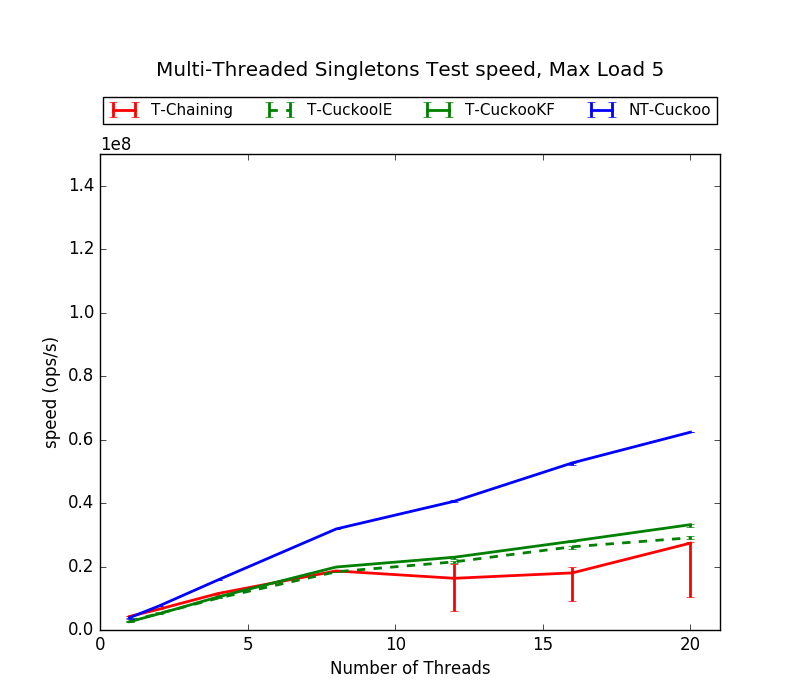
\includegraphics[height=2.25in]{maps/5HM1M:F34,I33,E33speed.png} &
        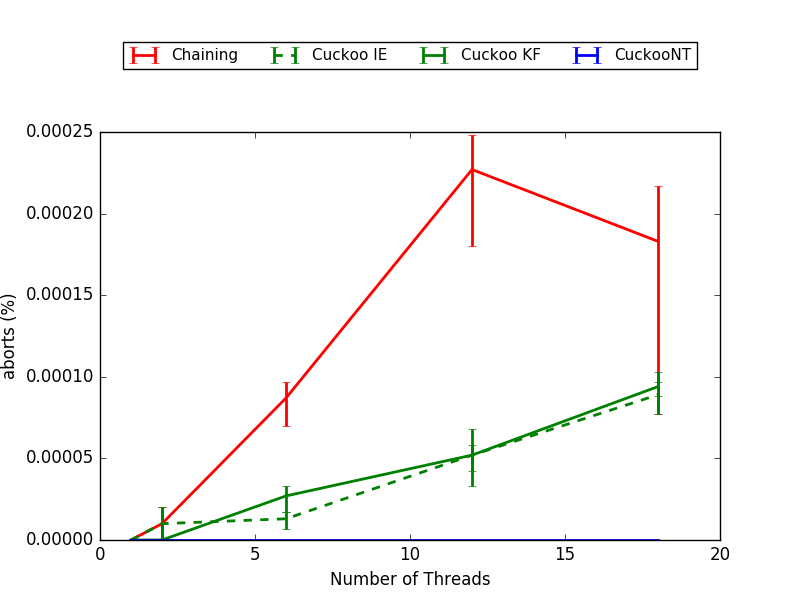
\includegraphics[height=2.25in]{maps/5HM1M:F34,I33,E33aborts.png}\\
        \hline 
        \multicolumn{2}{|c|}{{\footnotesize Maximum Load: 10}}\\
        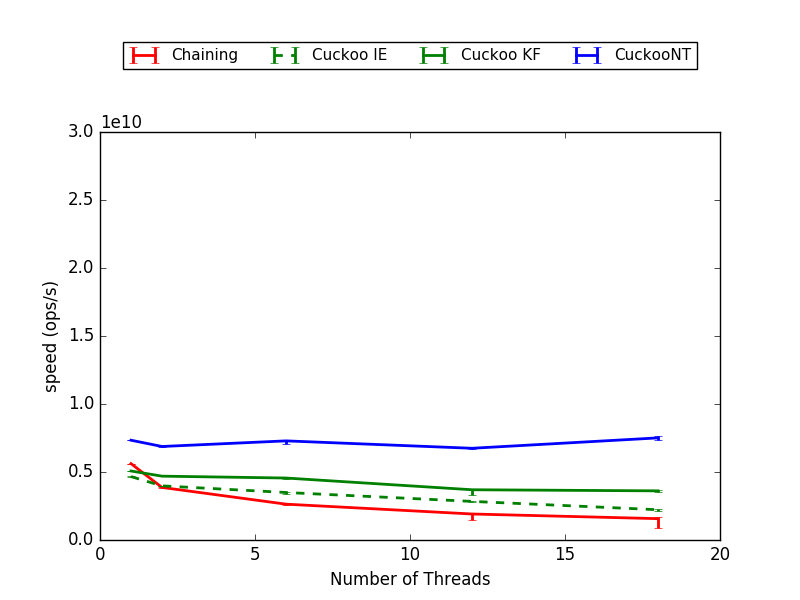
\includegraphics[height=2.25in]{maps/10HM1M:F34,I33,E33speed.png} &
        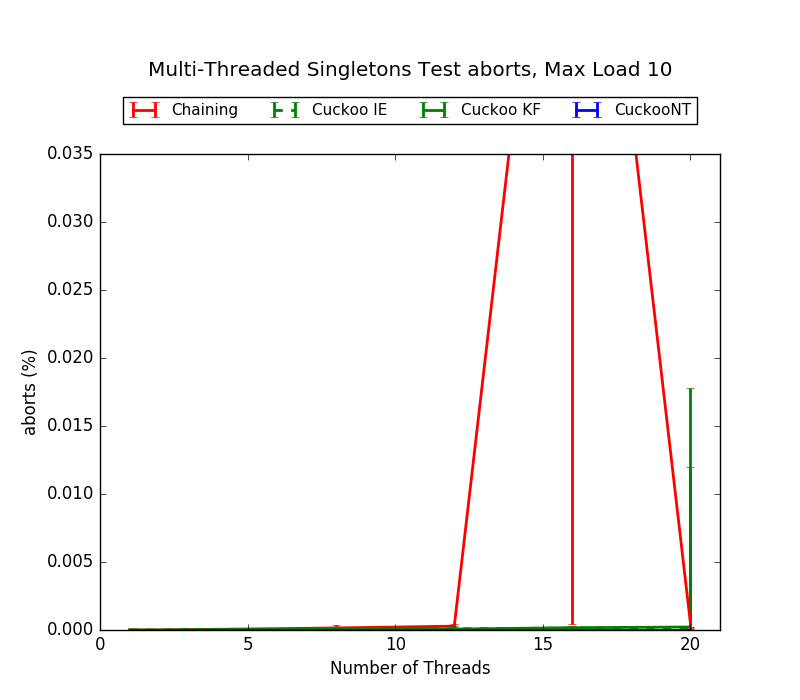
\includegraphics[height=2.25in]{maps/10HM1M:F34,I33,E33aborts.png}\\
        \hline 
        \multicolumn{2}{|c|}{{\footnotesize Maximum Load: 15}}\\
        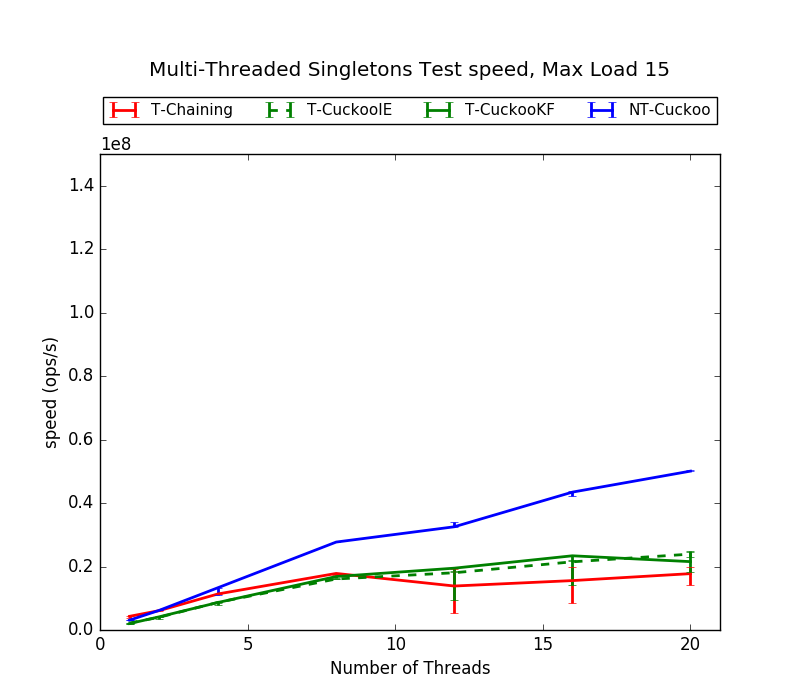
\includegraphics[height=2.25in]{maps/15HM1M:F34,I33,E33speed.png} &
    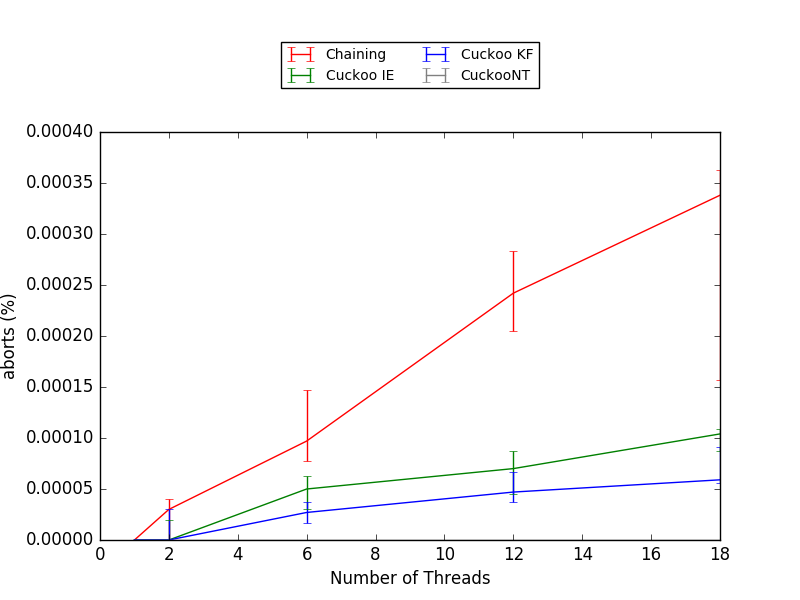
\includegraphics[height=2.25in]{maps/15HM1M:F34,I33,E33aborts.png}\\
    \hline 
    \end{tabular}
\label{fig:ntqueues}
\end{figure}
\begin{figure}[h!]
    \centering
    \caption{Hashmap Performance: 33\% Find, 33\% Insert, 33\% Erase, 125K Buckets}
    \begin{tabular}{|cc|}
        \hline 
        \multicolumn{2}{|c|}{{\footnotesize Maximum Load: 5}}\\
        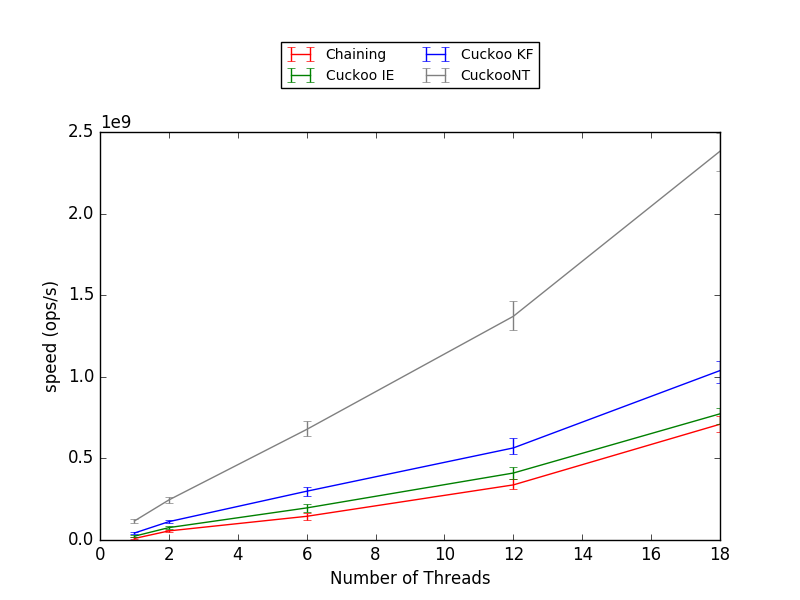
\includegraphics[height=2.25in]{maps/5HM125K:F34,I33,E33speed.png} &
        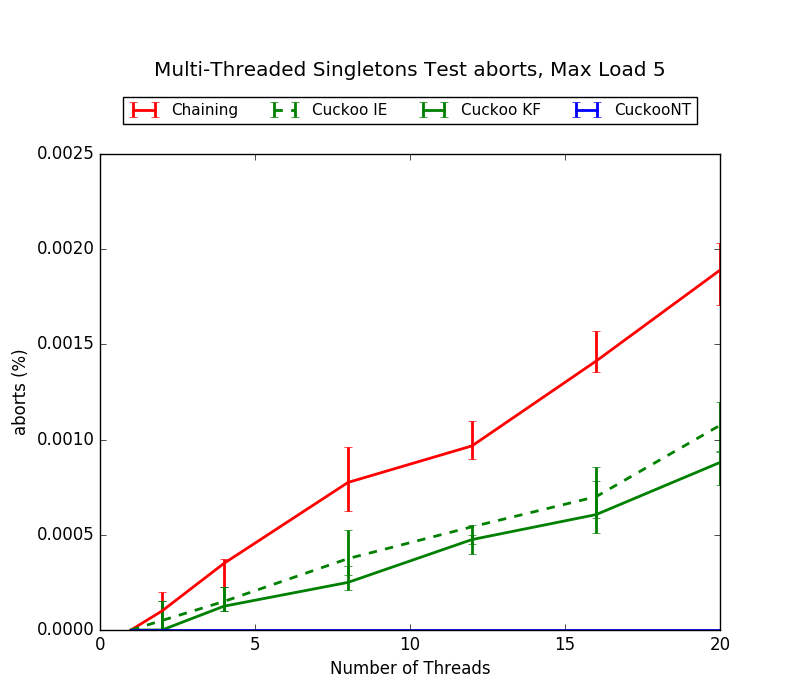
\includegraphics[height=2.25in]{maps/5HM125K:F34,I33,E33aborts.png}\\
        \hline 
        \multicolumn{2}{|c|}{{\footnotesize Maximum Load: 10}}\\
        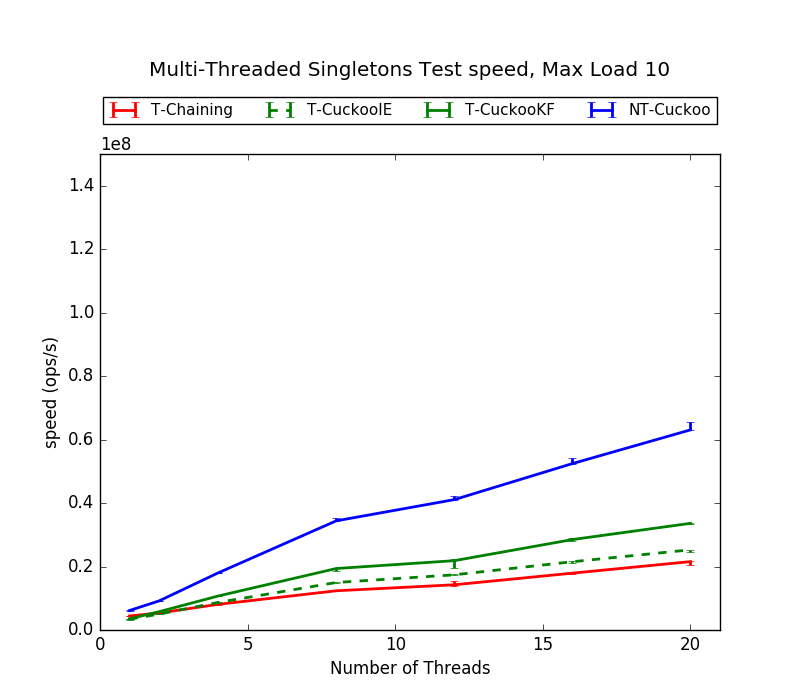
\includegraphics[height=2.25in]{maps/10HM125K:F34,I33,E33speed.png} &
        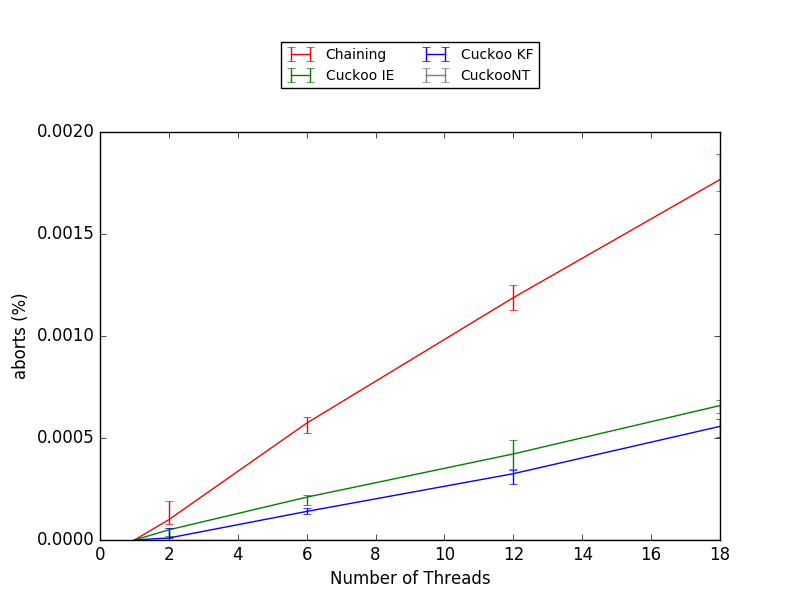
\includegraphics[height=2.25in]{maps/10HM125K:F34,I33,E33aborts.png}\\
        \hline 
        \multicolumn{2}{|c|}{{\footnotesize Maximum Load: 15}}\\
        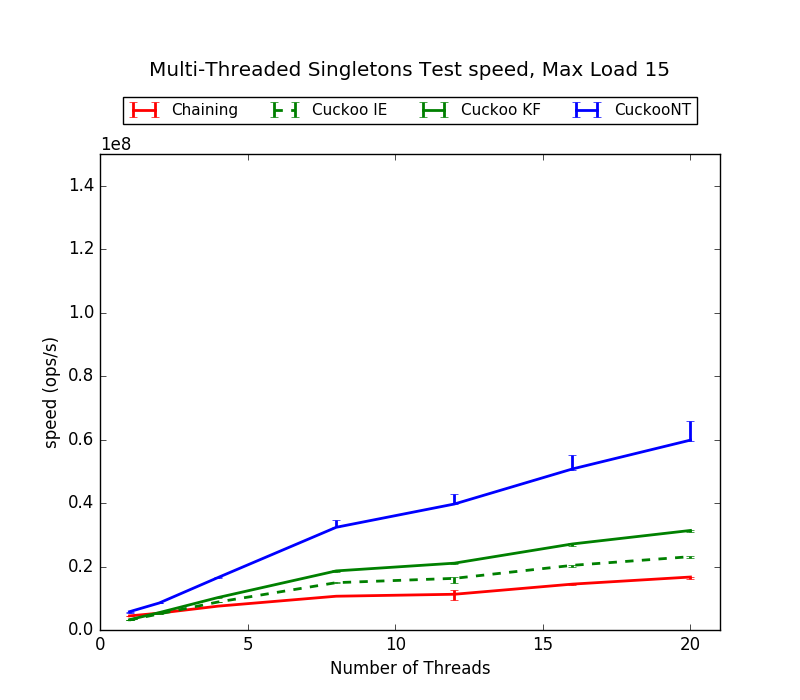
\includegraphics[height=2.25in]{maps/15HM125K:F34,I33,E33speed.png} &
    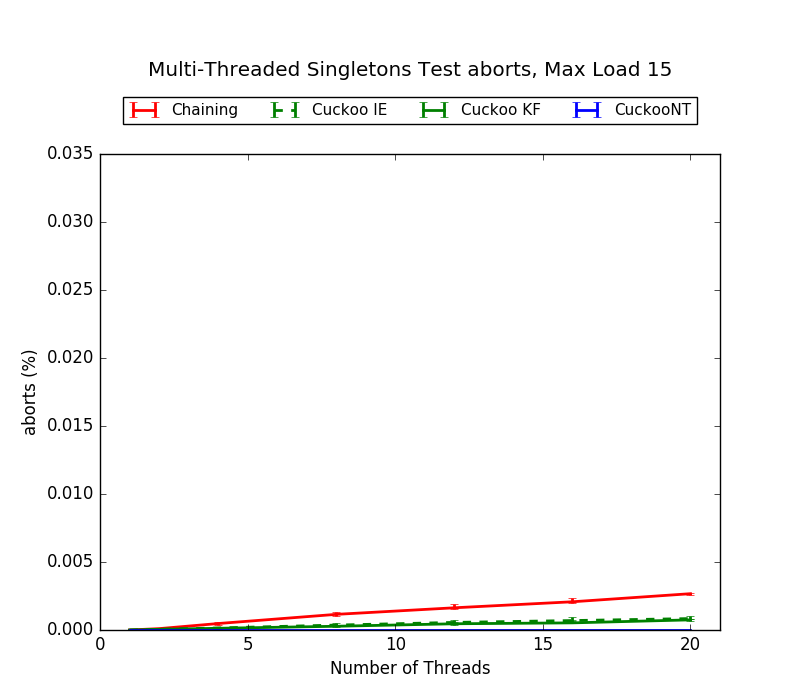
\includegraphics[height=2.25in]{maps/15HM125K:F34,I33,E33aborts.png}\\
    \hline 
    \end{tabular}
\label{fig:ntqueues}
\end{figure}
\begin{figure}[h!]
    \centering
    \caption{Hashmap Performance: 33\% Find, 33\% Insert, 33\% Erase, 10K Buckets}
    \begin{tabular}{|cc|}
        \hline 
        \multicolumn{2}{|c|}{{\footnotesize Maximum Load: 5}}\\
        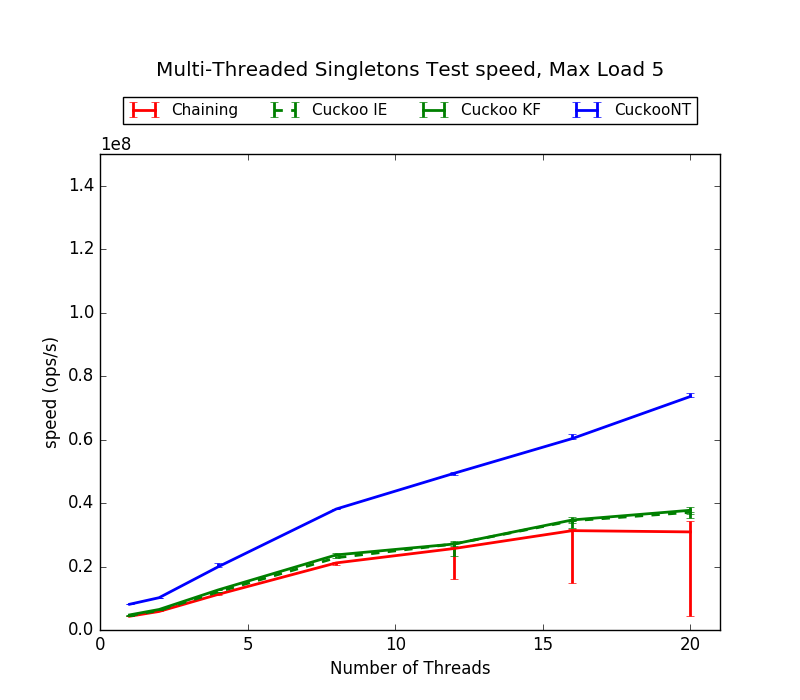
\includegraphics[height=2.25in]{maps/5HM10K:F34,I33,E33speed.png} &
        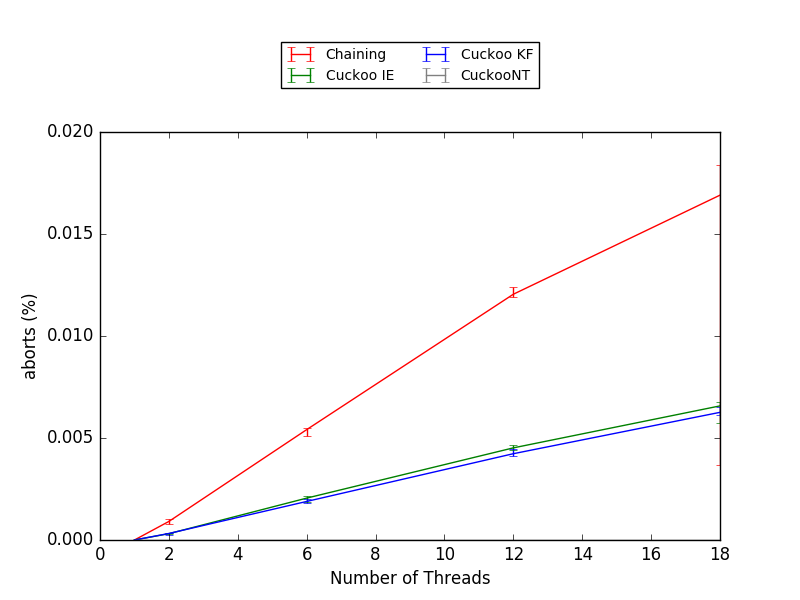
\includegraphics[height=2.25in]{maps/5HM10K:F34,I33,E33aborts.png}\\
        \hline 
        \multicolumn{2}{|c|}{{\footnotesize Maximum Load: 10}}\\
        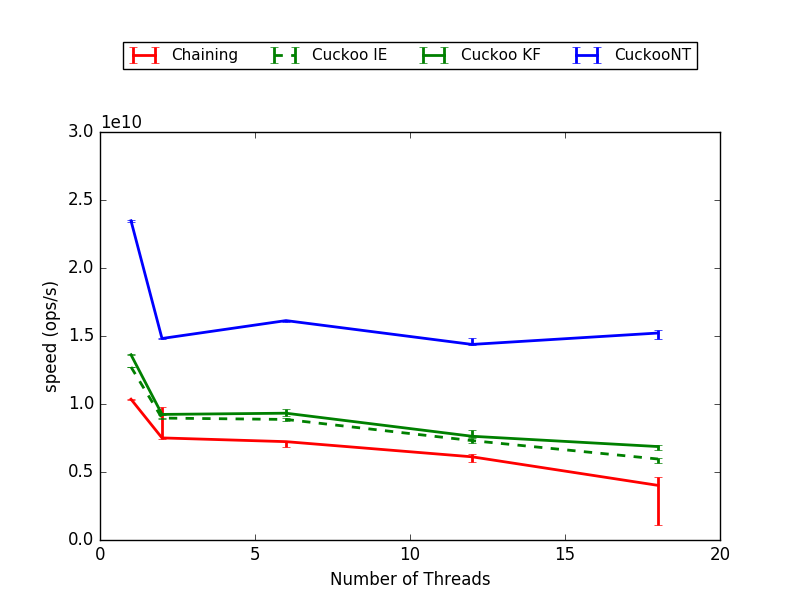
\includegraphics[height=2.25in]{maps/10HM10K:F34,I33,E33speed.png} &
        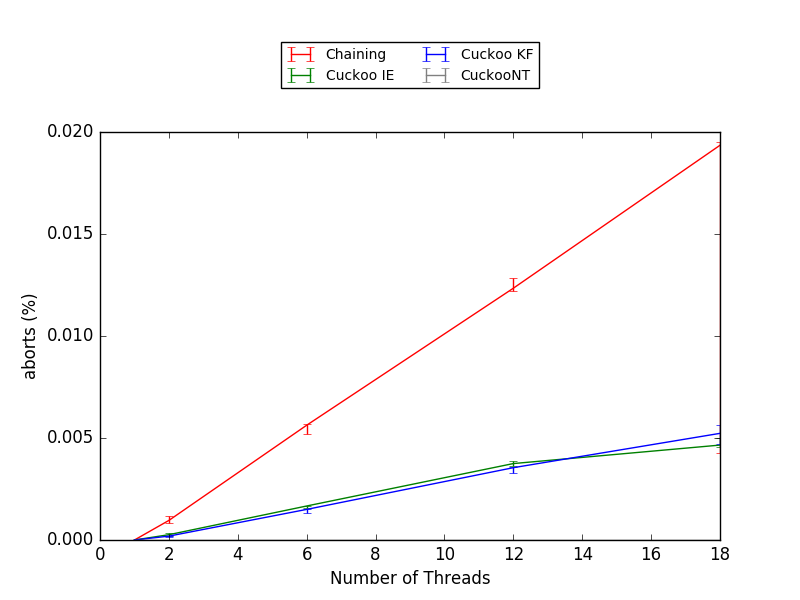
\includegraphics[height=2.25in]{maps/10HM10K:F34,I33,E33aborts.png}\\
        \hline 
        \multicolumn{2}{|c|}{{\footnotesize Maximum Load: 15}}\\
        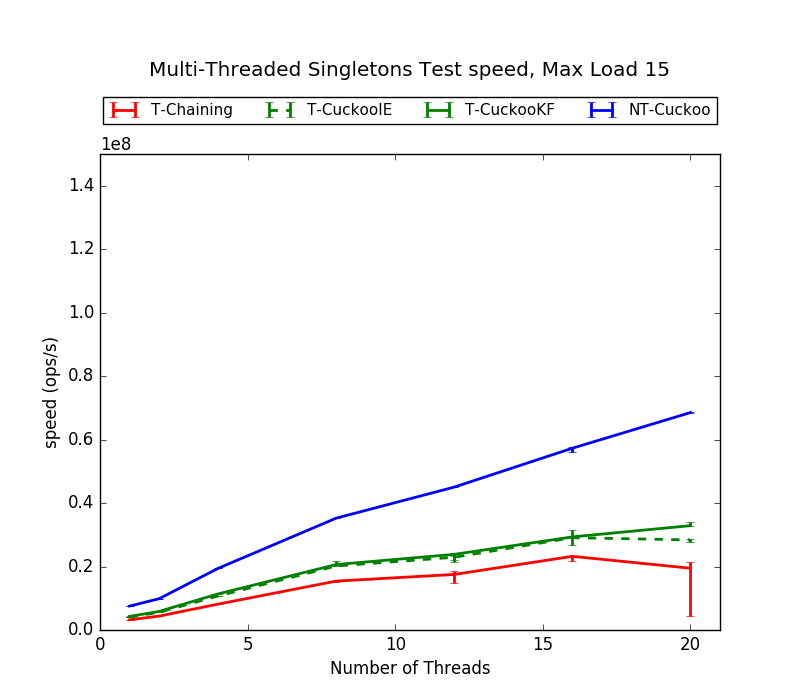
\includegraphics[height=2.25in]{maps/15HM10K:F34,I33,E33speed.png} &
    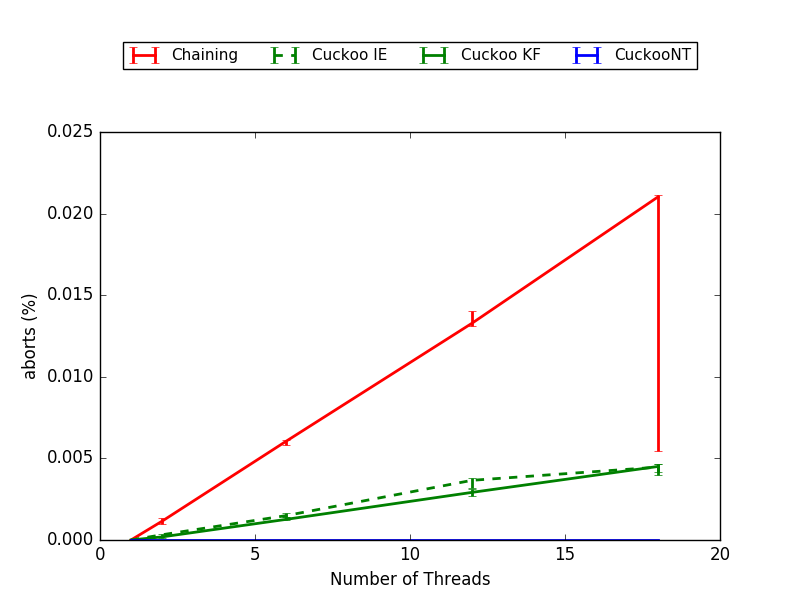
\includegraphics[height=2.25in]{maps/15HM10K:F34,I33,E33aborts.png}\\
    \hline 
    \end{tabular}
\label{fig:ntqueues}
\end{figure}
\begin{figure}[h!]
    \centering
    \caption{Hashmap Performance: 90\% Find, 5\% Insert, 5\% Erase, 1M Buckets}
    \begin{tabular}{|cc|}
        \hline 
        \multicolumn{2}{|c|}{{\footnotesize Maximum Load: 5}}\\
        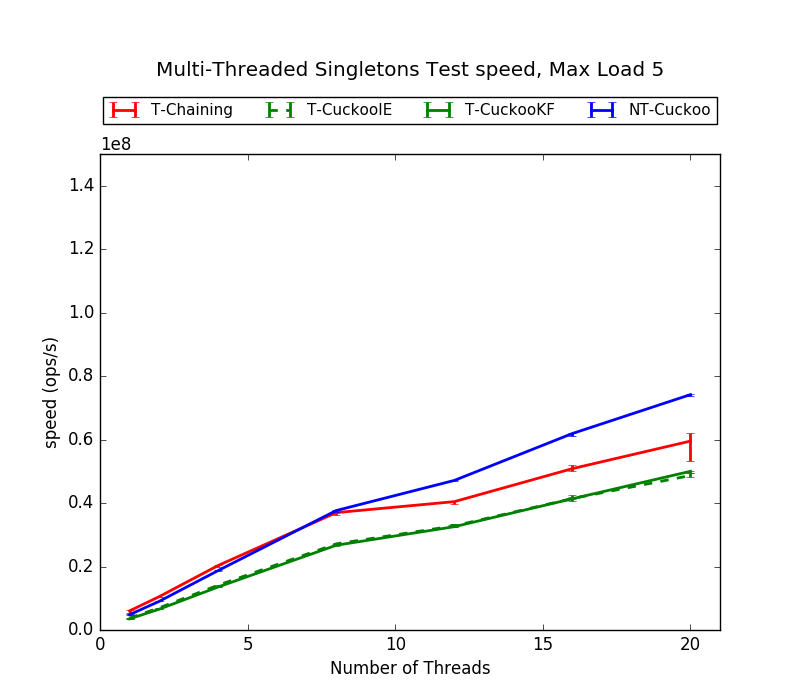
\includegraphics[height=2.25in]{maps/5HM1M:F90,I5,E5speed.png} &
        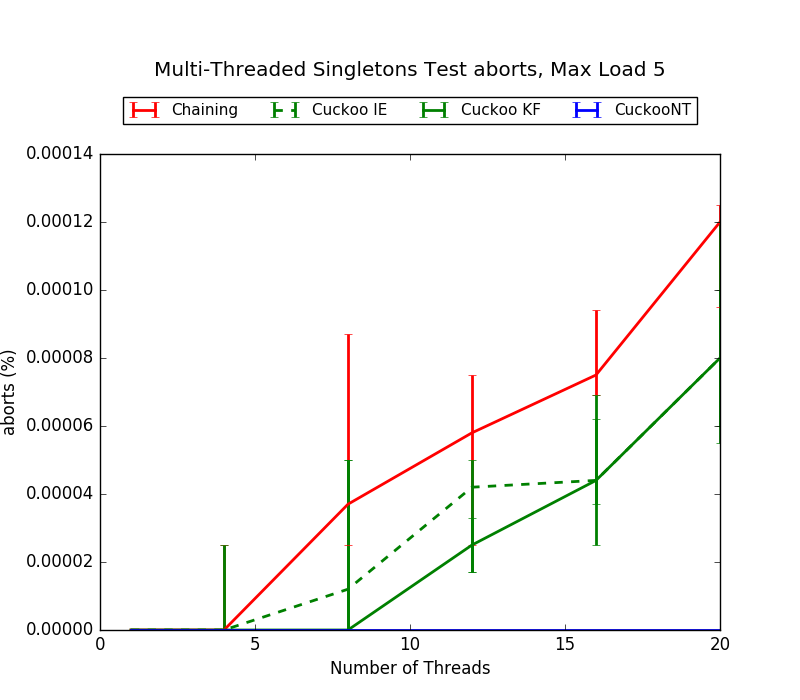
\includegraphics[height=2.25in]{maps/5HM1M:F90,I5,E5aborts.png}\\
        \hline 
        \multicolumn{2}{|c|}{{\footnotesize Maximum Load: 10}}\\
        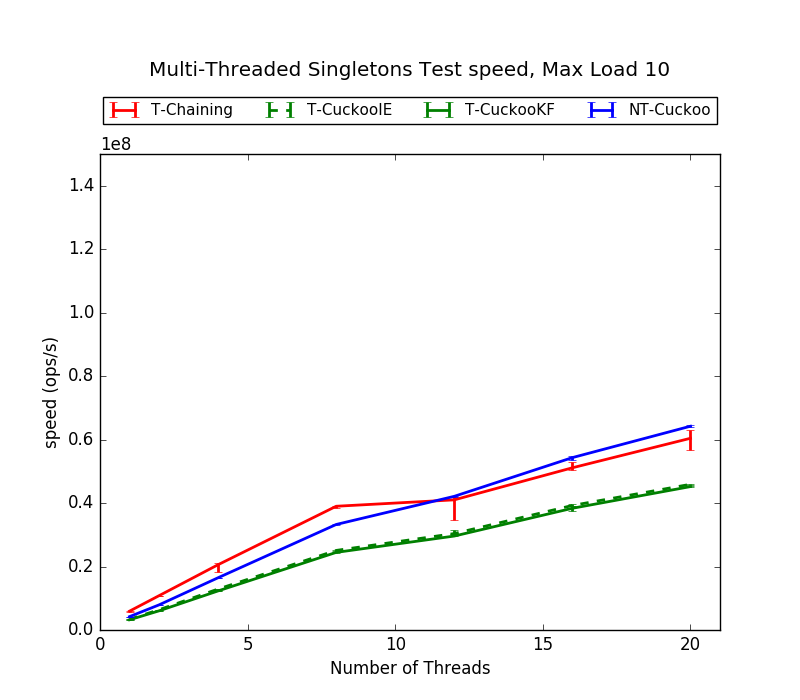
\includegraphics[height=2.25in]{maps/10HM1M:F90,I5,E5speed.png} &
        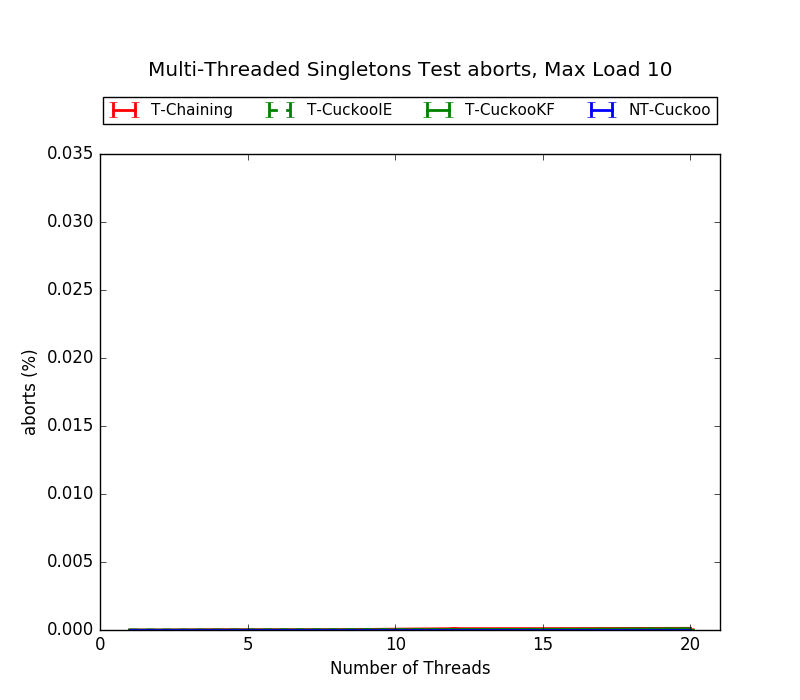
\includegraphics[height=2.25in]{maps/10HM1M:F90,I5,E5aborts.png}\\
        \hline 
        \multicolumn{2}{|c|}{{\footnotesize Maximum Load: 15}}\\
        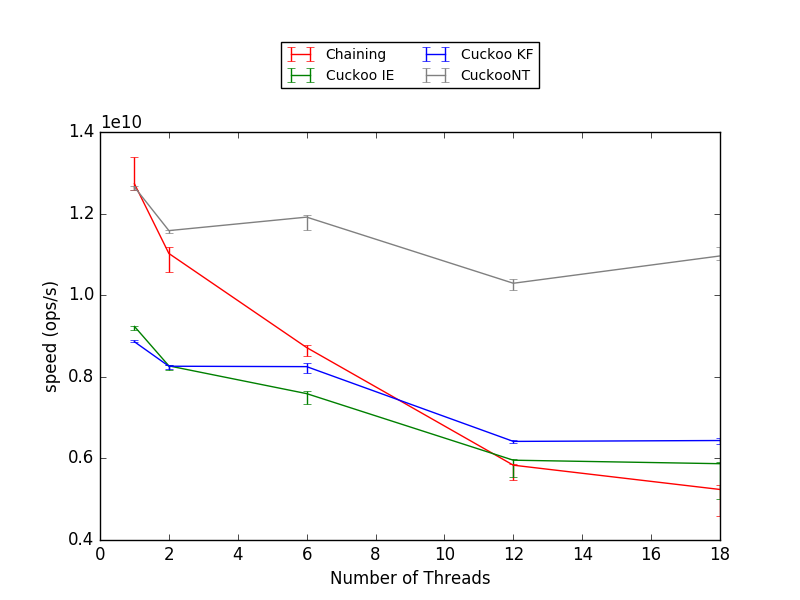
\includegraphics[height=2.25in]{maps/15HM1M:F90,I5,E5speed.png} &
        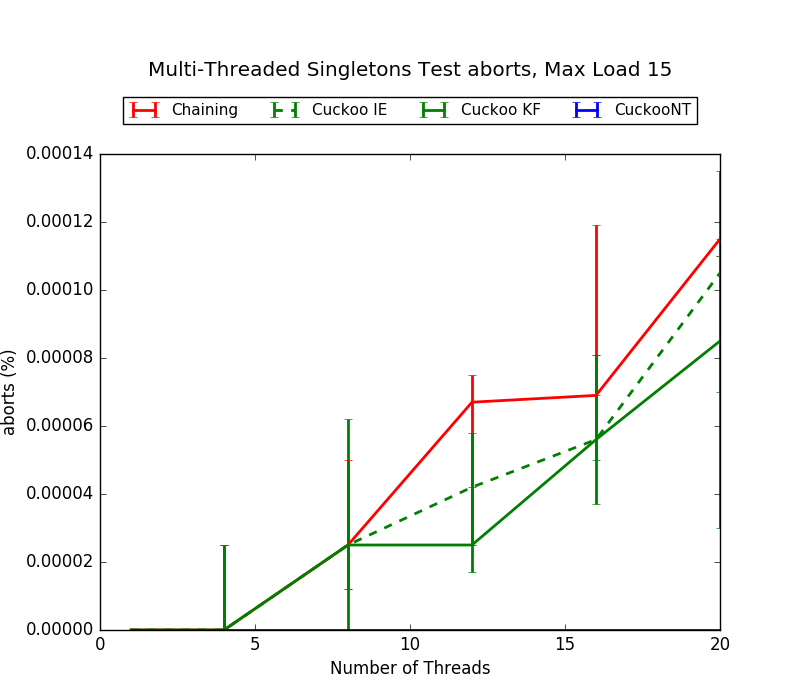
\includegraphics[height=2.25in]{maps/15HM1M:F90,I5,E5aborts.png}\\
    \hline 
    \end{tabular}
\label{fig:ntqueues}
\end{figure}
\begin{figure}[h!]
    \centering
    \caption{Hashmap Performance: 90\% Find, 5\% Insert, 5\% Erase, 125K Buckets}
    \begin{tabular}{|cc|}
        \hline 
        \multicolumn{2}{|c|}{{\footnotesize Maximum Load: 5}}\\
        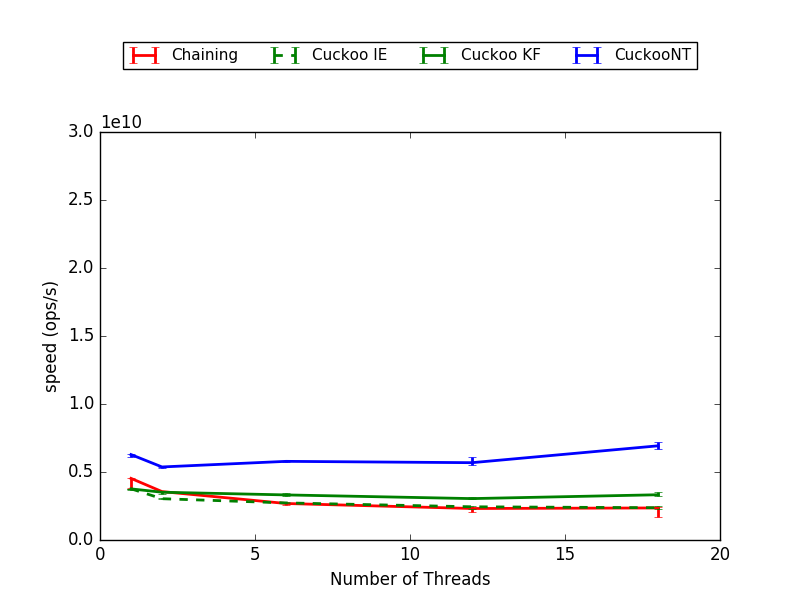
\includegraphics[height=2.25in]{maps/5HM125K:F90,I5,E5speed.png} &
        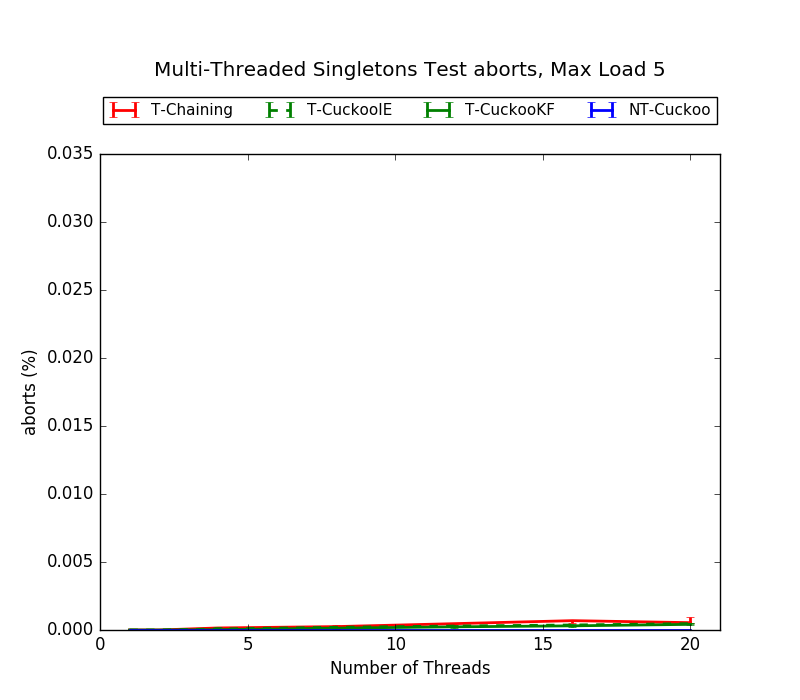
\includegraphics[height=2.25in]{maps/5HM125K:F90,I5,E5aborts.png}\\
        \hline 
        \multicolumn{2}{|c|}{{\footnotesize Maximum Load: 10}}\\
        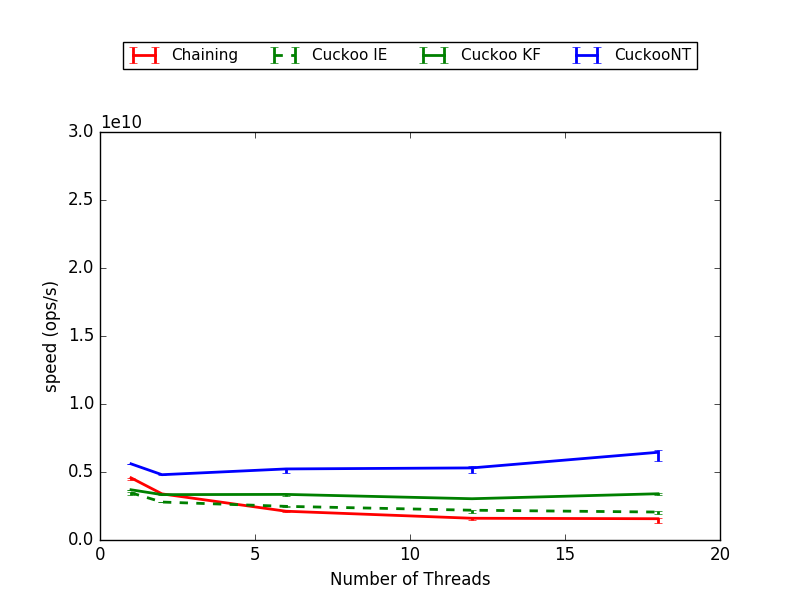
\includegraphics[height=2.25in]{maps/10HM125K:F90,I5,E5speed.png} &
        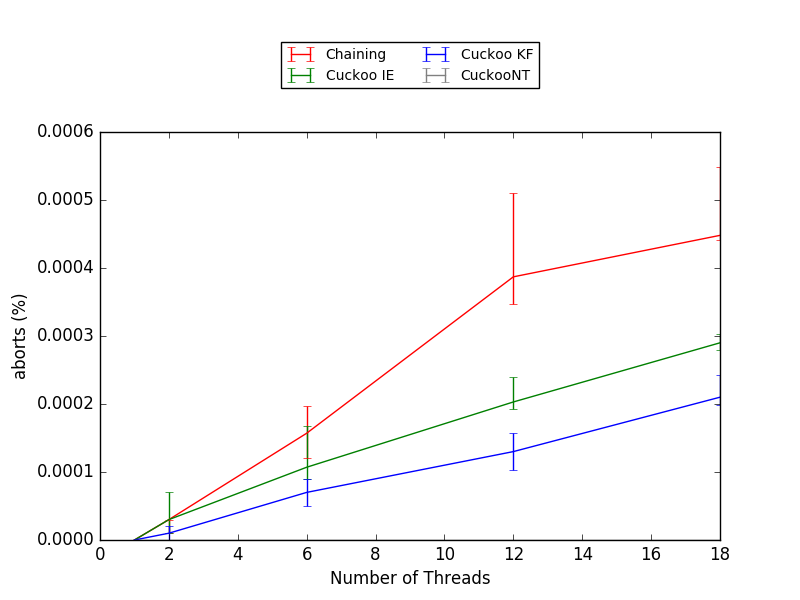
\includegraphics[height=2.25in]{maps/10HM125K:F90,I5,E5aborts.png}\\
        \hline 
        \multicolumn{2}{|c|}{{\footnotesize Maximum Load: 15}}\\
        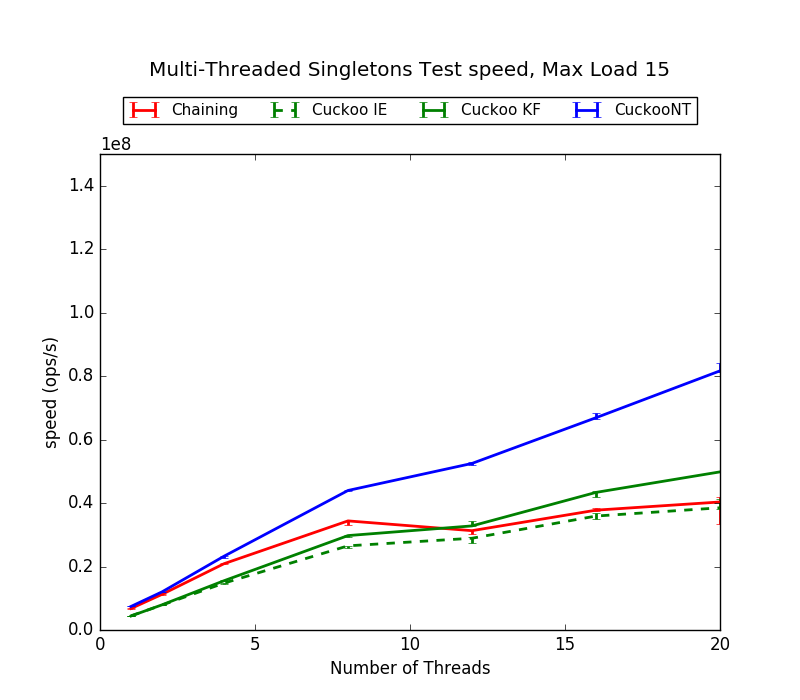
\includegraphics[height=2.25in]{maps/15HM125K:F90,I5,E5speed.png} &
        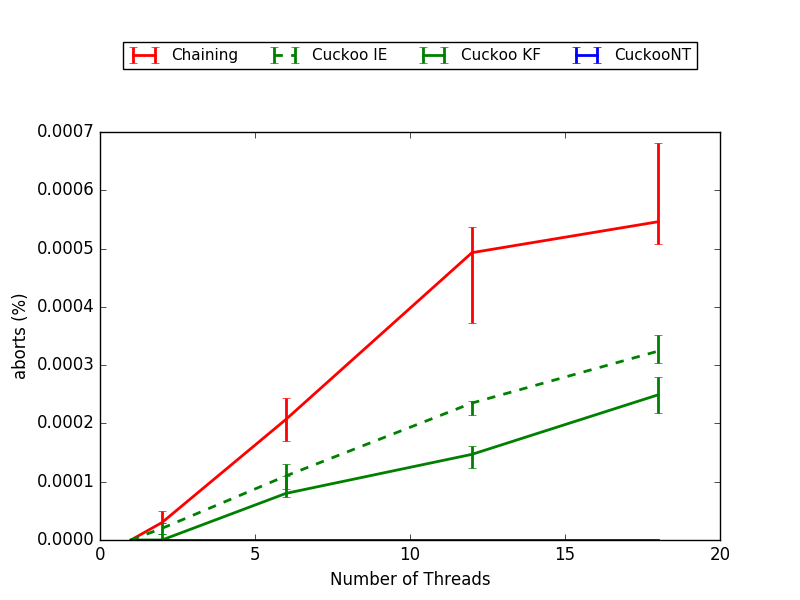
\includegraphics[height=2.25in]{maps/15HM125K:F90,I5,E5aborts.png}\\
    \hline 
    \end{tabular}
\label{fig:ntqueues}
\end{figure}
\begin{figure}[h!]
    \centering
    \caption{Hashmap Performance: 90\% Find, 5\% Insert, 5\% Erase, 10K Buckets}
    \begin{tabular}{|cc|}
        \hline 
        \multicolumn{2}{|c|}{{\footnotesize Maximum Load: 5}}\\
        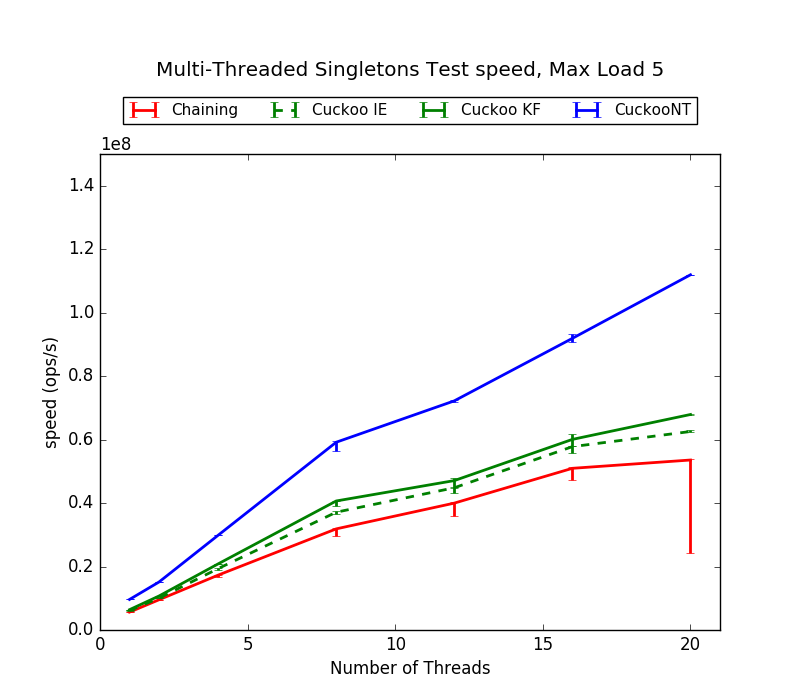
\includegraphics[height=2.25in]{maps/5HM10K:F90,I5,E5speed.png} &
        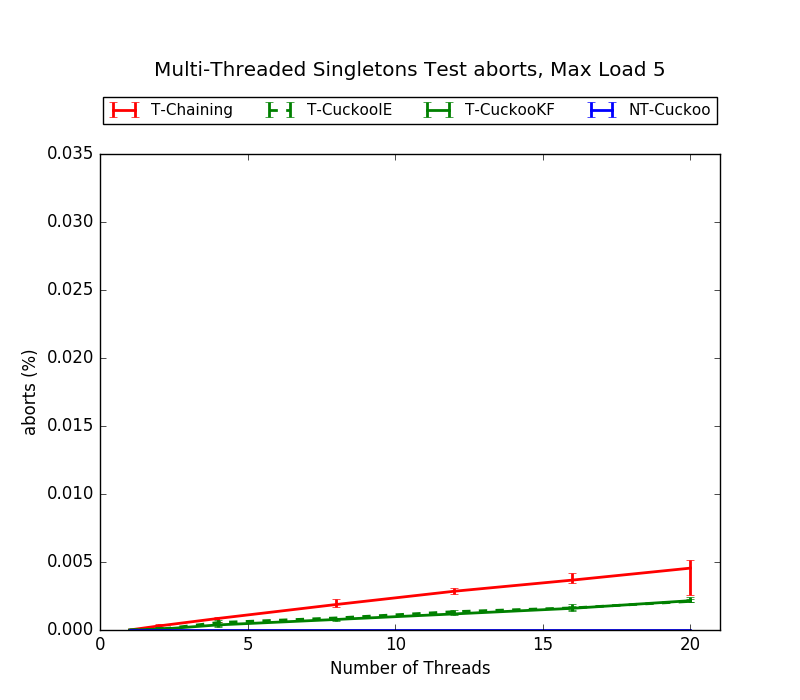
\includegraphics[height=2.25in]{maps/5HM10K:F90,I5,E5aborts.png}\\
        \hline 
        \multicolumn{2}{|c|}{{\footnotesize Maximum Load: 10}}\\
        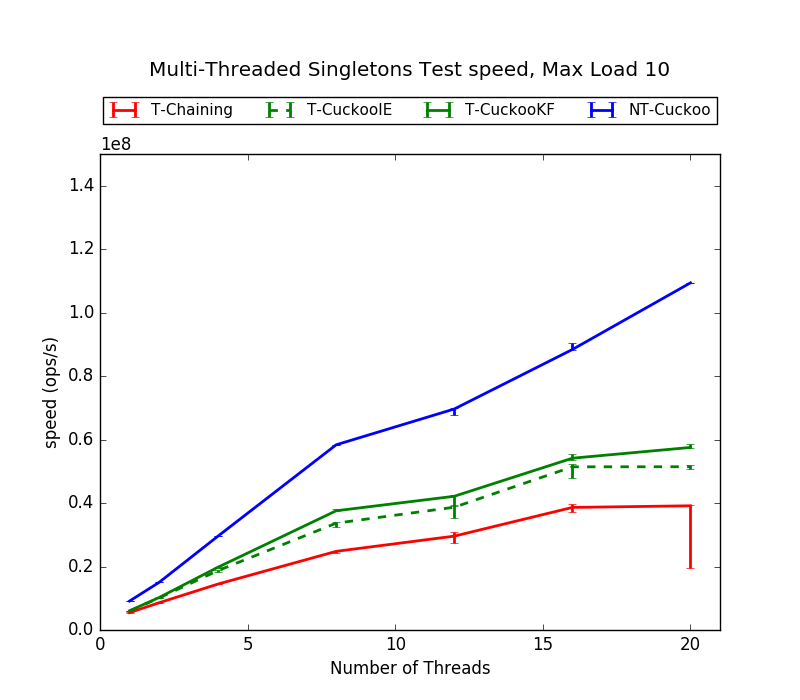
\includegraphics[height=2.25in]{maps/10HM10K:F90,I5,E5speed.png} &
        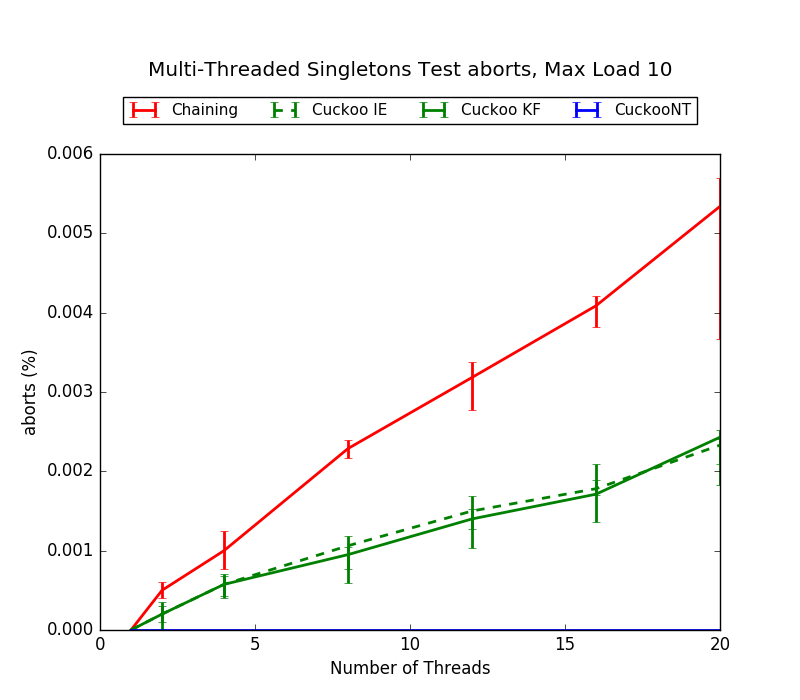
\includegraphics[height=2.25in]{maps/10HM10K:F90,I5,E5aborts.png}\\
        \hline 
        \multicolumn{2}{|c|}{{\footnotesize Maximum Load: 15}}\\
        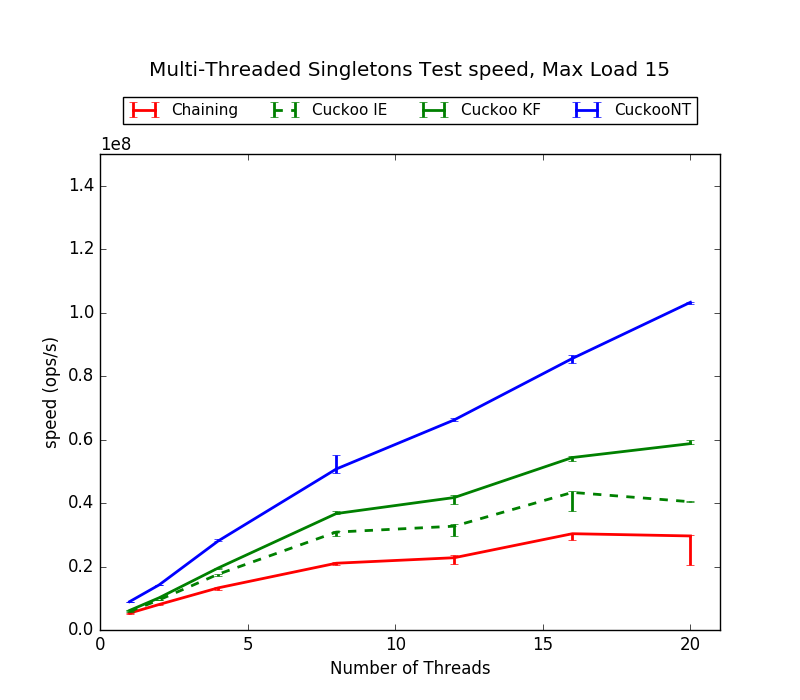
\includegraphics[height=2.25in]{maps/15HM10K:F90,I5,E5speed.png} &
    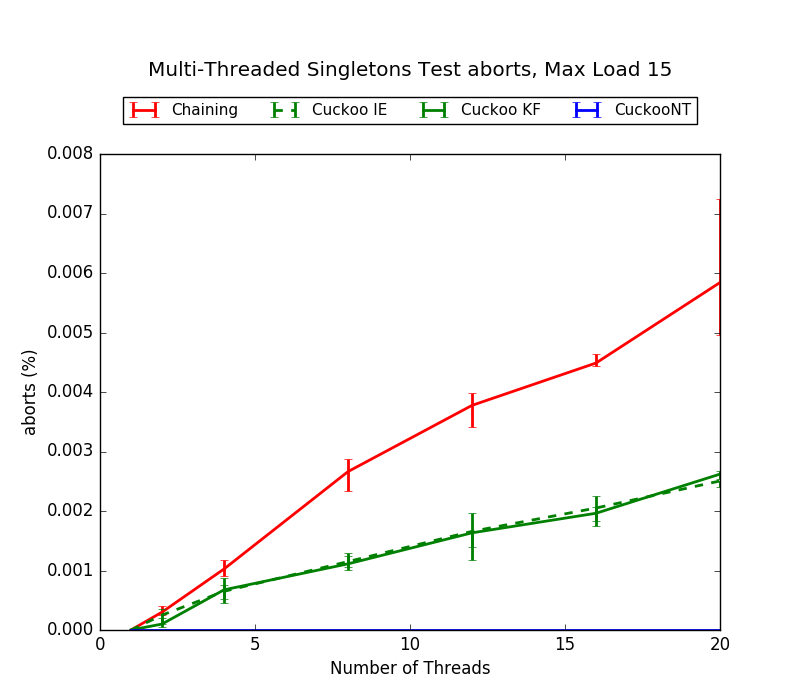
\includegraphics[height=2.25in]{maps/15HM10K:F90,I5,E5aborts.png}\\
    \hline 
    \end{tabular}
\label{fig:ntqueues}
\end{figure}


\floatstyle{plain} 
\restylefloat{figure}
\begin{figure}[ht!]
    \caption{Hashmap Cache Misses}
    \centering
    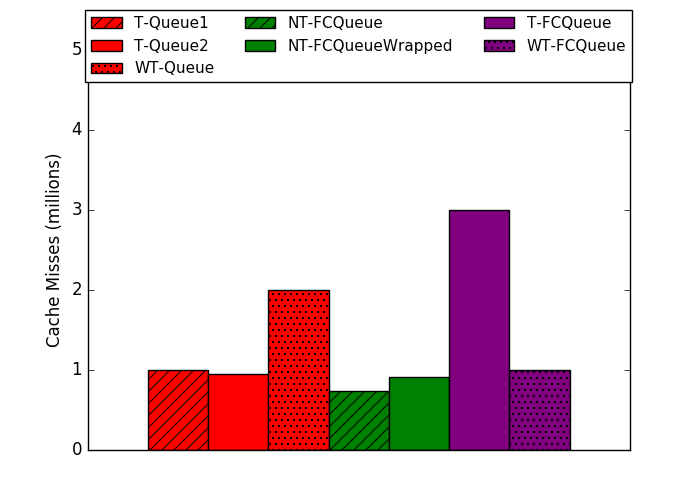
\includegraphics[height=3in]{fcqueues/cm.png}
    \label{fig:cm_maps}
\end{figure}


\iffalse
\begin{table}[h!]
    \centering
\begin{tabular}{|c|c|c|c|c|c|}
    find(x)-find(x) & insert(x)-insert(x) & erase(x)-erase(x) & find(x)-insert(x) & find(x)-erase(x) & insert(x)-erase(x)\\
    \hline
    & W-W, W-R & W-W, W-R & R-W & R-W & W-W, W-R
\end{tabular}
    \caption*{R-R relations are not shown.}
    \caption{Dependencies of pairs of hashmap operations}
    \label{table:hashmapsimpledeps}
\end{table}
\fi
